% !Mode:: "TeX:UTF-8"
% !TEX program  = xelatex

%\documentclass{cumcmthesis}
\documentclass[withoutpreface,bwprint]{cumcmthesis} %去掉封面与编号页,电子版提交的时候使用。


\usepackage[framemethod=TikZ]{mdframed}
\usepackage{url}   % 网页链接
\usepackage{subcaption} % 子标题
\usepackage{rotfloat,makecell}
\usepackage{framed}
\usepackage{gbt7714}

\lstset{
    breaklines
}

\title{基于Q型聚类分析的二手房价多元线性回归模型}
\tihao{B}
\baominghao{XJ22007}
\schoolname{西安交通大学}
\membera{苏悦馨}
\memberb{孙思雨}
\memberc{张卓立}
\supervisor{XXX}
\yearinput{2022}
\monthinput{07}
\dayinput{03}

\begin{document}%符号转化,归一化化成标准化

\maketitle

\begin{abstract}%这是摘要
    为响应“房子是用来住的,不是用来炒的”精神定位,西安政府出台相关政策促进房屋流通,结合房屋交易“淡旺季”的市场规律,西安二手房价格会产生一定程度的波动。本文依据西安2993套二手房的相关数据,通过建立基于Q型聚类分析的多元线性回归模型,分析了房屋梯户比、面积等11项因素对西安二手房价的影响,预测了政策出台后下一年二手房价与成交量变动走势,能够为有不同需求的市民家庭在选购二手房的过程中提供参考性意见。
   
    针对任务一,需要分析房屋各项指标对单价的贡献占比。首先,我们收集了西安市内2993套二手房关于11个有效指标的相关数据,采用层次分析法将其中一些定性指标通过判断矩阵量化,同时将一些定量指标归一化,实现预处理。再利用主成分分析法找出有效指标的主因子。从MATLAB绘制的离散点图中,我们发现归一化后的单价呈条带状聚集、带内线性关系显著,故可利用Q型聚类分析将样本点分成多个聚类,对每一聚类分别建立多元线性回归模型,这样就找出了每一项指标对房屋单价的具体贡献大小。 最后结合对家庭结构的分析依据模型结果,针对不同家庭的住房需求提出相应的购房建议。
    
    针对任务二,要求进行模型的评估与改进。首先,我们在原数据集内进行分层抽样,以抽取到具有代表性的9个小区为样本,将样本相关指标数据进行标准化赋值。再在原有模型中代入数值,通过求解主因子变量找到小区数据所属聚类,再由聚类内线性回归模型得到5月份房价预测值。
    
    考虑到任务一模型对交易月份不敏感,结合实际房价波动的年周期性,我们引入三角形式的函数模型,求解得出改进后的模型。此外,通过分析抽样小区被商圈、学区、景区的覆盖情况,得出地理因素对二手房单价的正向影响。这就说明以附件中的行政区平均房价占比作为地理因素的归一化赋值的合理性,进而能够实现模型的再改进。
    
    针对任务三,我们结合西安政府的相关政策,逐条分析其中可能会对二手房价造成影响的因素。再根据收集到的近两年房价随时间变动数据,利用对数曲线预测下一年中西安二手房的价格波动趋势。进而通过房价变动定性预测、分析政策对于二手房成交量的影响。
   
    综上,本文由数据驱动,对样本划分后的各个聚类分别建立多元线性回归模型,直观地展现了影响西安二手房价格的多项指标所占比重,再以具有代表性的9个小区为样本进行验证,对于研究影响二手房价格的市场波动与政策驱动具有良好的适用性。

  \textbf{关键字:} 层次分析法,主成分分析, Q型聚类分析, 多元线性回归模型,对数曲线预测法。

\end{abstract}

\section{问题重述}
%地理位置,建筑年代,朝向,高低,户型,面积
\subsection{问题背景}
华商报指出,5月西安新建商品住宅销售价格环比上涨0.3\%,二手住宅销售价格环比下降0.4\%。其中,新房价格涨幅相比上月有小幅提高。今年前5个月里,西安1月新房价格没有变化,2、3月分别上涨1\%、0.4\%,4月份涨幅回落到0.2\%,5月上涨0.3\%,同时5月西安新房市场整体呈现平销局面。
而在5月28日晚,西安政府出台政策调整商品住房交易,包括但不限于涉及降低限购门槛、缩短限售时间。随后,市面上涌入大量新房房源。预计6月西安新房供应量可能达到上半年供应新高。
另外我们发现,西安二手房价格走势与新房价格走势的差异加剧。西安二手房价格继4月环比下降0.1\%后,在5月份环比下降0.4\%。分产品来看,5月份西安90$m^2$及以下、90-144$m^2$及144$m^2$以上二手房价格分别环比下降0.1\%、0.5\%和0.5\%。
\subsection{问题提出}
西安二手房数据中心的最新统计数据表明:市民选购二手房时更偏重考虑地理位置,而在户型方面三居室则是首选。具体表现为:市民选购二手房时往往更倾向于离地铁近、附近有超市和学校、近市区的房型,并且受到浏览关注的主要户型是三居室,5居室以上的户型受关注度低。此外还应考虑购房用途,如果购房不是用来自住,地理位置更好的房屋往往具有更大的升值空间,更适于投资。
西安二手房市场房源众多,找到影响二手房价格的因素有利于购房者根据需求有效甄别并作出合理的选择。

任务一:根据所给网站显示的西安在售二手房信息和附件提供的相关数据,建立数学模型,分析影响西安二手房价格的因素,为有意购买二手房的家庭提供建议。

任务二:查找西安二手房5月份的多项数据指标,检验任务一求解的模型的合理性,并加以改进。 

任务三:西安市政府于5月底出台“西安关于调整商品住房交易政策有关问题的通知”,预测这项通知政策将对二手房价产生的影响,分析并预测未来一年内西安二手房价和成交量的走势。
\section{问题分析}
本文要解决西安二手房价格影响因素分析问题。任务一、二要求根据收集到的西安二手房价格波动、地理位置、户型面积等相关数据建立不同因素对房价影响的数学模型、收集并代入5月份的数据检验评估模型的准确性,根据模型的反应情况,在原有模型基础上加以改进。任务三要求我们结合西安政府的相关政策,预测分析下一年中二手房价格与成交量的变动趋势。

经过分析,我们得出问题解决流程图如下:
\begin{figure}[H]
    \centering
    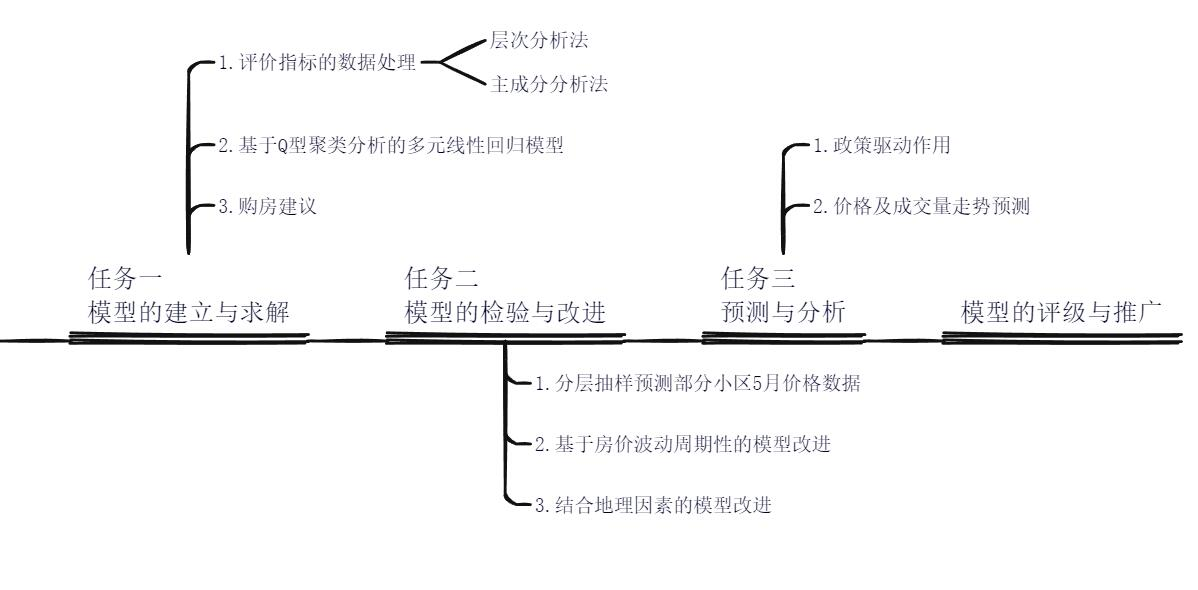
\includegraphics[scale=0.45]{流程图.jpg}
    \caption{问题解决流程图}
    \label{fig:问题解决流程图}
\end{figure}

\subsection{任务一的分析}
针对任务一,为充分分析房屋各项指标对单位平方米房屋价格的精准贡献占比,我们先收集了西安市内2993套二手房关于11个有效指标的相关数据,采用层次分析法将其中一些定性指标通过判断矩阵量化,同时将一些定量指标归一化,保证随着其中任一项指标数值的增大房屋单价均得到提升。紧接着我们采用主成分分析法找出三个线性无关的主因子,计算它们的表达式中有效指标的系数。下面我们需要确定以这三个主因子为自变量的房屋价格表达式。

考虑到样本数量较大,我们不妨将其按Q型聚类分析分成多个集类。利用MATLAB进行数值分析后,我们通过观察归一化后的房屋单价,发现样本点在图中的分布明显呈16个条带状,且每个条带中样本点均有明显的线性关系,这就说明了对每个集类进行多元线性回归拟合的合理性。

最后由预处理后的房屋数据,结合主因子表达式,对每一聚类分别建立多元线性回归模型,这样就找出了每一项指标对房屋单价的具体贡献大小。

此外,再根据模型结果与对家庭结构的分析,针对不同家庭的购房需求提出相应的指导性建议。
\subsection{任务二的分析}
针对任务二,我们先在原数据集内进行分层抽样,选取有代表性的9个小区作为样本,并且将样本相关指标数据进行标准化赋值。在原有模型中代入处理后的数据,通过求解主因子变量找到所属聚类,再由聚类内线性回归结果分别预测对应小区的五月份房价。

由于原先模型中指标随时间变动不大,因此在改进模型时需加入对时间变量的考量。我们增添“月份”这一自变量,结合房价波动的年周期性,考虑引入余弦波动因子,求解得出改进后的模型。再代入样本小区的数据,发现加上时间波动项后模型得到了有效改进。

此外,我们通过分析抽样小区被商圈、学区、景区的覆盖情况,得出地理因素对二手房单价的影响,即“被重点区域覆盖程度程度越高,房屋单价普遍越高”。这就说明了能够以附件中的行政区平均房价作为地理因素的归一化赋值,并将这项指标加入模型的考量,实现模型的再改进。

\subsection{任务三的分析}
针对任务三,我们结合西安政府的相关政策,逐条分析其中可能会对二手房价造成影响的因素,同时根据收集到的房价随时间变动数据,利用对数曲线预测下一年中西安二手房的价格波动趋势。进而通过房价变动走势,结合经济学相关原理,预测未来一年内二手房成交量的变动趋势。

\section{假设条件}
1.仅考虑下述三个方面共11项主要因素对于西安二手房价的影响:房屋自身因素(包括:梯户比,面积,总价格,楼层高度,房屋朝向,装修状况,供暖方式,抵押信息,户型),地理因素,交易月份。这些因素涵盖了市民购房时主要关注的指标,也具有足够多的对应数据支撑。

2.假设针对不同方向的政策通知之间不会相互干扰。

3.假设新政策通知的实施不受其他阻力影响,下一年中政策不会中断受阻。

4.假设新冠疫情等不可抗力因素对消费者二手房的购买意愿造成的影响可以忽略不计。

5.假设二手房交易对二手房市场平稳。
\section{符号说明}
\begin{table}[H]
    \centering\small
    \begin{tabular}{cp{8cm}<{\centering}c}
    \toprule
    符号 & 描述 & 单位\\
    \midrule
        $m_i\ (i=1,\cdots,8)$ & 每个单位化或标准化后的评价指标 & / \\
        $\beta_i\ (i=1,2,3)$ & 每个主成分 & /\\
        $s$ & 二手房面积 & $m^2$\\
        $m_S$ & 样本所有小区中最小二手房面积 & $m^2$\\
        $M_S$ & 样本中所有小区最大二手房面积 & $m^2$\\
        $c$ & 二手房每平方米价格 & 元$/m^2$\\
        $c_{\min}$ & 样本二手房中最小每平方米价格 &元$/m^2$\\
        $c_{\max}$ & 样本二手房中最大每平方米价格 & 元$/m^2$\\
        $CI$ & 一致性指标 & /\\
        $RI$ & 平均随机一致性指标 & /\\
        $CR$ & 一致性比例 & /\\
        $n$ & 小区数目 & 个\\
        $b_i$ & 第$i$个小区 & /\\
        $t$ & 月份 & 月\\
    \bottomrule
    \end{tabular}
\end{table}
\section{任务一:模型的建立与求解}

\subsection{评价指标的数据处理}
针对一些定性指标如“房屋朝向、供暖方式”和一些定量指标如“梯户比、面积”,我们需要先对数据进行预处理:首先确立评价体系,将定性指标量化,这一过程中保证在其他因素不变的前提下,随单一指标变量的增大,二手房单位平方米单价上升:其次将指标单位化转换为$[0,1]$之间的数值或进行标准化处理;接着通过层次分析法确立判断矩阵,为不同指标打分;最后对于得分进行主成分分析,将成分矩阵旋转实现正交化,就能确定主因子表达式。这就求解了不同因素对于西安二手房的具体影响贡献大小。
\subsubsection{层次分析法}
由于二手房价的影响因素分层交错,且其中既包括定性指标又包括定量指标,为了量化分析不同因素造成的影响比重,我们首先采用层次分析法这一评价方法,通过对不同方面的影响程度大小进行打分,得到判断矩阵,继而实现影响指标的量化。


结合网站查找到的西安六月份二手房相关数据,我们综合考虑以下影响因素:\\
1.梯户比
2.面积
3.总价格
4.楼层高度
5.房屋朝向
6.装修状况
7.供暖方式
8.抵押信息
9.户型
10.地理因素
11.交易月份

这些指标可以大致分为三类:房屋自身因素(1$\sim$9),地理因素,交易月份。

在第一问中,我们只需要利用6月份的西安二手房相关数据,故无需考量交易月份带来的影响,且由于地理因素与房屋本身状况无关,且地理因素对房屋单价产生的影响与其他因素相比大得多,因此需要我们在下一部分“模型的检验与改进”中进行单独考量。

首先,我们考虑梯户比,即“房屋电梯数/住户数”。由于这一数据介于0,1之间,且在控制变量的条件下,随着这一数值的增加,房屋每平米单价升高,这相当于这项数据已经天然的完成了归一化处理,我们将得到的数据记为$m_1$。

其次我们考虑面积。由于不同城区中不同小区的楼盘面积是固定的,这就决定了一定时间内每个小区的二手房的面积是固定的。为了便于接下来的主成分分析,首先我们将这项数据进行归一化处理,设所有小区面积的最小值是$m_S$,最大值是$M_S$,小区的面积是$s$,则做处理如下
\begin{equation}
    s'=\frac{s-m_S}{M_S-m_S},
\end{equation}
即可归一化数据,我们将得到的数据记为$m_2$.

再考虑总价格。我们对价格数据进行归一化处理,设房屋总价格为$c$,所有小区中的最低总价为$c_{\min}$,最高总价为$c_{\max}$,则有
\begin{equation}
    m_3=\frac{c-c_{\min}}{c_{\max}-c_{\min}}.
\end{equation}

然后考虑楼层高度。我们将房屋楼层分为低中高三类,分类的评价指标大致相同,例如在较低楼层房屋中主要以低、中层为主,而较高楼层房屋则兼具低、中、高三种。下面进行层次分析.判断矩阵如下:(列从左往右按照低中高楼层)
\begin{equation}
    A_2=\begin{bmatrix}
        1 & 2 &3 \\
        1/2 & 1 &2\\
        1/3 & 1/2 & 1
    \end{bmatrix}.
\end{equation}
得到单位化后评分$m_4=(0.540059,0.296736,0.163205)$,
$CR=CI/RI=0.0079<1$,通过一致性检验。

接着考虑房屋朝向。我们在量化这一指标的过程中综合考虑传统观念与地理因素,具体来讲,由于中国人“南北为正”的传统观念加上西安所处地理位置位于北半球,气候以南北风向为主的特点,通常南北朝向的房屋更为通透,采光与通风条件都更好。依此类推,西安房屋的朝向优劣顺序大致为南、东南、东、西南、北、西,其中朝南最好,朝西最差。下面考虑东西南北四个朝向,进行层次分析,判断矩阵如下:(从左到右是东西南北)
\begin{equation}
    A_3=\begin{bmatrix}
        1 & 3 & 1/2 & 2\\
        1/3 & 1 & 1/6 & 1/2\\
        2 & 6 & 1 & 3\\
        1/2 & 2 & 1/3 & 1
    \end{bmatrix}.
\end{equation}
单位化后评分$m_5=(0.267206,0.082996,0.495951,0.153846)$,
$CR=-0.0202<1$,通过一致性检验。

再考虑装修状况。西安二手房可以分为精装,简装,毛坯三种,同样进行层次分析。判断矩阵如下:(从左到右分别是精装,简装,毛坯)
\begin{equation}
    A_4=\begin{bmatrix}
    1 & 2 &3\\
    1/2 & 1 & 2\\
    1/3 & 1/2 & 1
    \end{bmatrix}.
\end{equation}
单位化得到评分$m_6=(0.540059,0.296736,0.163205)$,
$CR=0.0079<1$,通过一致性检验。

然后考虑供暖方式。相比于集中供暖,自供暖不受供暖时间限制,且可以实现温度自主调节,单位立方米取暖耗气量更低更为节能,因而相对评分更高。
故当集中供暖时取$m_7=1/3$,自供暖时取$m_7=2/3$。

接下来考虑抵押信息。房屋交易分为有无抵押两种情况,我们假设有抵押时抵押额度对二手房的价格影响不大。记有抵押时$m_8=2/3$,无抵押时$m_8=1/3$。

最后我们考虑户型。由于主要户型分为一、二、三、四、五居室,且根据国家统计局2020年数据显示,现阶段我国平均家庭规模为2.92人。此外,家庭结构组成以夫妻家庭和三口之家的核心家庭为主,因此购买者群体中有三居室需求的比重更大,市场对于三居室需求量更高,这与题干信息“市民浏览关注的主要户型是三居室”相吻合。而户型因素往往由购房需求直接决定,购房需求又与家庭结构密切相关,因而这一因素不参与主成分分析,将在“购房建议”中将进行单独讨论。


\subsubsection{主成分分析法}
主成分分析法是将$n$维空间上的数据通过降低噪声等方式降低维度,事实上,处理后的维度上仍存在足够的有效信息,并不会造成关键信息的丢失。

在上面的部分中,我们已经完成了对于在链家网站\cite{RN2}上找到的西安全城共2993套二手房屋数据信息的预处理,得到各个指标归一化后的数值。事实上,通过相关性矩阵我们发现一些指标之间存在较强的相关性。
\begin{figure}[H]
\centering
    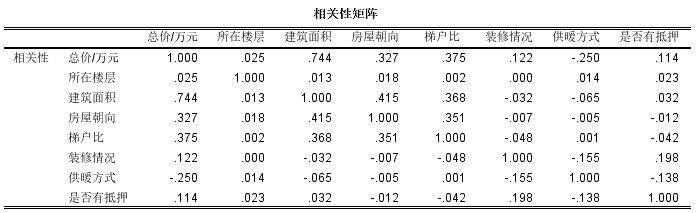
\includegraphics[scale=0.8]{相关性矩阵.png}
    \caption{相关性矩阵}
    \label{fig:相关性矩阵}
\end{figure}
下面对于上述指标,采用主成分分析法先消去它们之间的相关性,再确定它们对于房价的影响权重。记西安市每个小区是$b_{i},i=1\cdots,n$,评价指标是$m_1,\cdots,m_8$, $b_i$的每个评价指标对应的数据$x_{i1},\cdots,x_{i8}$,假设$b_i$的每个数据对应权重$a_{ij},j=1,\cdots,8$.令$\bm{x}=\frac{1}{n}\sum_{i=1}^n\bm{x}_i=(\bar{x}_1,\cdots,\bar{x}_8)^T$,$\bm{x}_i=(x_{i1},\cdots,x_{i8})^T$.最后用主成分分析,得到$b_i$的特征值
\begin{equation}
    y_i=a_{i1}x_{1}^\ast+\cdots+a_{i8}x_{8}^\ast=a_i^Tx^\ast.
\end{equation}
其中$x_i^\ast$是中心化后的数据:$x_j^\ast=x_j-\bar{x}_j$.

先仅考虑房屋自身因素对房屋每平方米价格的影响,房屋价格随月的波动以及随地理位置的变化将单独考虑。将得到的三个主因子与附件中提供的房屋价格数据进行拟合,我们可以得到评分与每平米房价的关系如下:

\begin{figure}[H]
    \centering
    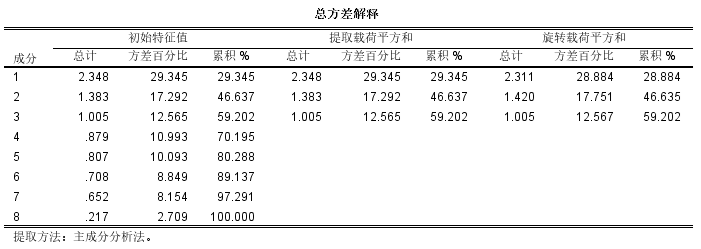
\includegraphics[scale=0.8]{总方差解释.png}
    \caption{总方差解释}
    \label{fig:总方差解释}
\end{figure}
同时根据各个指标的特征值大小,绘制碎石图如下:
\begin{figure}[H]
    \centering
    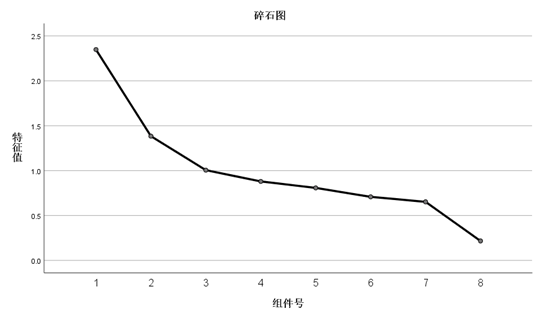
\includegraphics[scale=0.7]{碎石图.png}
    \caption{碎石图}
    \label{fig:碎石图}
\end{figure}
由于前三项成分对应的特征值均大于1,且累计贡献率较高,故我们可以从上述八项房屋自身因素中提取出这三种作为主因子,继而可以得到成分矩阵。需要注意的是,这里仅能保证主因子之间的线性无关性,并不能保证它们相互正交。因而再进行旋转变换,使得主因子之间相互正交,得到旋转后的成分矩阵如下:

\begin{figure}[H]
    \centering
    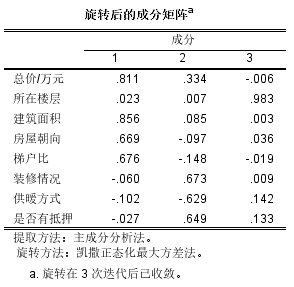
\includegraphics[scale=1.1]{旋转后的成分矩阵.png}
    \caption{旋转后的成分矩阵}
    \label{fig:旋转后的成分矩阵}
\end{figure}
图中给出了我们不同指标在主成分中的载荷,表中的每一个载荷量都表示主成分与对应指标的相关系数。以第一列为例,第一列中正数对应的指标在成分一上有较高载荷,说明成分一基本反映了这些指标的信息。以此类推,现有的三个主因子基本反映了原有八项指标信息,实现了数据降维与线性无关化处理。

因此,记第$i$个主因子为$\beta_{i}$,我们可以得到三个主因子表达式:
\begin{gather}
   \beta _{1}=0.811m_{1}+0.023m_{2}+0.856m_{3}+0.669m_{4}+0.676m_{5}\\
   \beta _{2}=0.334m_{1}+0.007m_{2}+0.085m_{3}+0.673m_{6}+0.649m_{8}\\
   \beta _{3}=0.983m_{2}+0.003m_{3}+0.036m_{4}+0.009m_{6}+0.142m_{7}+0.133m_{8}
\end{gather}
                                    
\subsection{基于Q型聚类分析的多元线性回归模型}

Q型聚类分析是对多个样本进行定量分类的多元统计分析方法,应用于本题背景下,能有效实现对2993个西安二手房数据样本点的分类处理。
\begin{figure}[H]
    \centering
    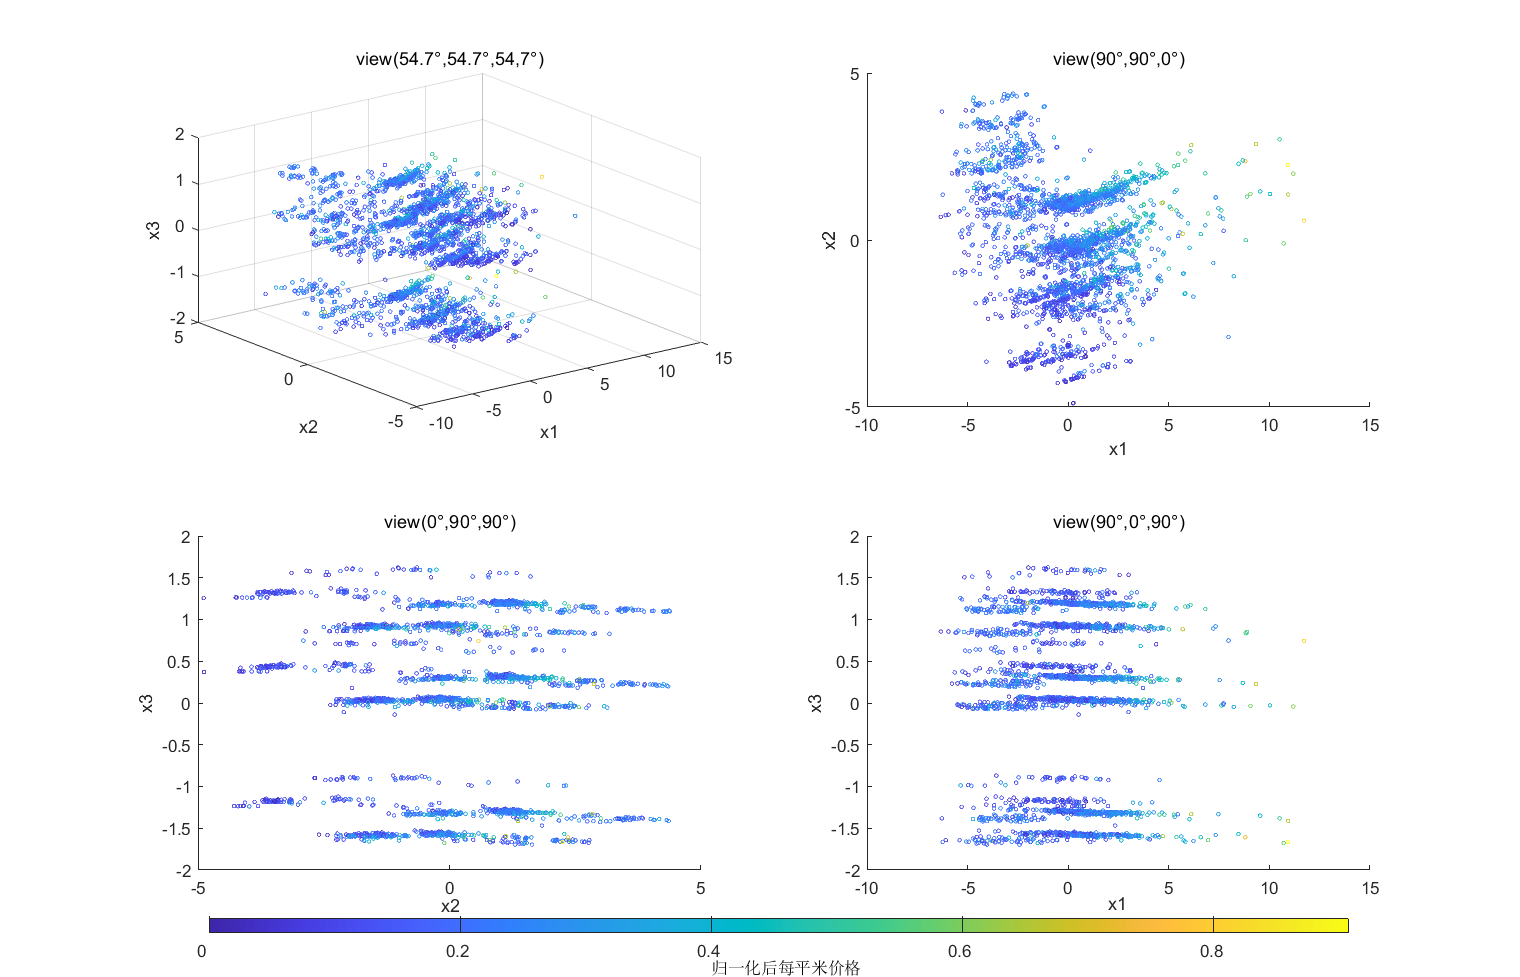
\includegraphics[scale=0.35]{不同角度的样本点分布图.png}
    \caption{样本点分布图}
    \label{样本点分布图}
\end{figure}
通过图6:样本点分布图,可以发现,样本点在$\mathbb{R}^3$空间内呈条带状聚集分布。而样本点的颜色代表其价格,在不同聚类内,样本点颜色的变化都有近似相同的规律。

这表明我们可以根据不同聚类划分样本,并对于每一个样本集类分别建立相应的多元线性回归模型。由于这样的模型选择与实际样本分布高度吻合,因此模型的拟合性能很强。



具体步骤展开如下:

   首先计算$n$个样本点两两之间的欧几里得距离$d_{ij}$,记为矩阵$D=(d_{ij})_{n\times n}$;
  接着构造$n$个类,使得每个类中仅包含一个样本点,以保证每一类的平台高度均为0;
    其次合并距离最近的两类为新类,并且以这两类间的距离值作为聚类图中的平台高度;
    最后计算新类与当前各类的距离,若类的个数已经等于1,则绘制聚类图,否则继续执行上述操作。
    这样操作后就能确定样本类的个数和不同分类。

    \newpage
    \vfill
我们绘制的样本点Q型聚类图如下,依据该聚类图,我们将样本点分为16个聚类。
\vfill
\begin{figure}[H]
    \centering
    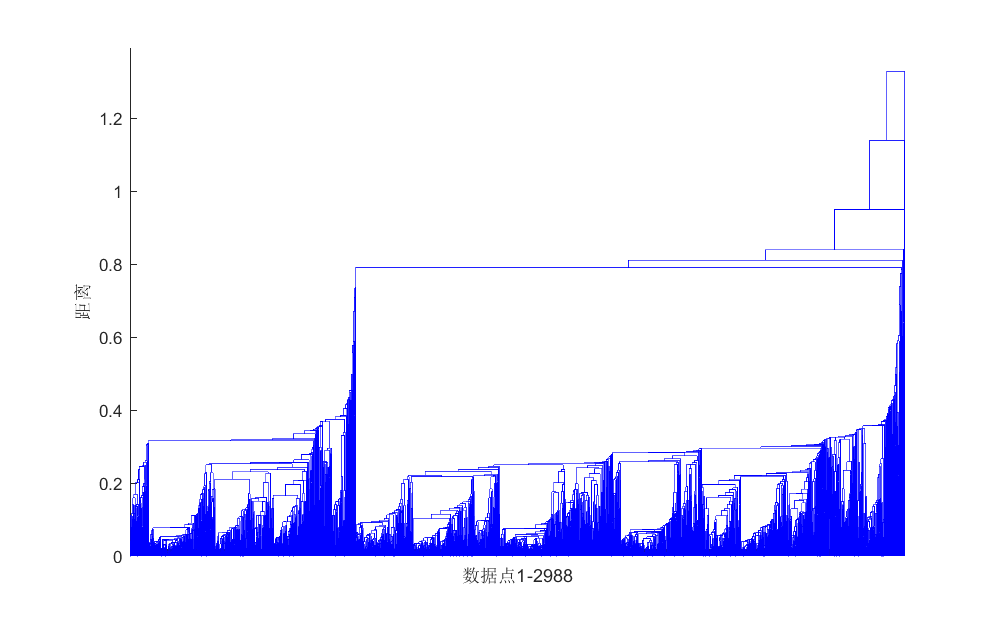
\includegraphics[scale=0.6]{样本点的Q型聚类图.png}
    \caption{样本点的Q型聚类图}
    \label{fig:样本点的Q型聚类图}
\end{figure}

\begin{paragraph}{}
    下面我们准确计算模型结果。首先将西安2993套二手房屋的原始数据标准化,即减去均价再除以其标准差,得到8项房屋自身因素的总体情况/标准化赋值。其次将这些数据代入上文求出的主因子表达式,得到对应的三项主因子变量值,分别将其记为$x_i$(i=1,2,3)。再根据Q型聚类分析得到的16个不同聚类,分别代入相关指标数据进行多元线性回归拟合,求解
\begin{equation}
    c_i=\beta _{1}x_{1}+\beta _{2}x_{2}+\beta _{3}x_3+\beta _{0}
\end{equation}
得到每个聚类对应的参数,这就是最终的多元线性回归模型。
\end{paragraph}
\vfill
\newpage
\begin{table}[H]
    \centering
    \small
      \begin{tabular}{cccccc}
      \toprule
        \multirow{2}*{\makecell{Q型聚类所属\\聚类编号}}&\multicolumn{5}{c}{该聚类内线性回归结果}\\
        \cline{2-6}
        &$\beta_0$& $\beta_1$ & $\beta_2$ & $\beta_3$ & $R^2$\\
      \midrule
      1     & 6791.75200  & 4497.77131  & 899.55426  & 25.48512  & 0.77670  \\
      2     & 4557.41988 & 3976.84814  & 1515.36989  & 17.74094  & 0.57866  \\
      3     & 14188.20214  & 2012.83502  & 690.56700  & 0.46038  & 0.94577  \\
      4     & 32571.22315  & 3134.05042  & 1058.81008  & 110.22048  & 0.98221  \\
      5     & 70092.34112  & 3374.12419  & -674.82484  & 0.41805  & 0.88342  \\
      6     & 16317.13320  & 2801.81189  & -128.36238  & 56.41085  & 0.55221  \\
      7     & -1389.35010  & 3156.33470  & 861.66694  & 402.23966  & 0.45779  \\
      8     & 6801.92236  & 3078.65218  & 1422.13044  & 594.59976  & 0.69121  \\
      9     & 5247.84812  & 4321.72800  & 2304.34560  & 0.31656  & 0.81334  \\
      10    & 79124.50235  & 2900.88000  & -580.17614  & 171.51998  & 0.78175  \\
      11    & 75930.02041  & 5637.16800  & 1127.43461  & 144.46382  & 0.99741  \\
      12    & -291.47920  & 3406.38811  & 105.27762  & 150.06802  & 0.99311  \\
      13    & -2469.73312  & 3052.52582  & -178.50516  & 288.20160  & 0.91572  \\
      14    & 11278.60613  & 2905.66440  & 581.13288  & 288.50832  & 0.44301  \\
      15    & 943.29199  & 4197.21163  & 839.44233  & 132.06852  & 0.67081  \\
      16    & 5001.91320  & 3054.38429  & 34.87738  & 0.67722  & 0.99458  \\
      \bottomrule
      \end{tabular}%
    \caption{聚类内线性回归结果}
  \end{table}%
  其中$R^2$表示相关系数,其值越接近1表明模型拟合效果越好,

\subsection{购房建议}
\subsubsection{依据家庭需求}
任务一要求为我们为有意购买二手房的家庭提供建议,而家庭成员的数量往往决定了对于二手房的户型需求,因此我们首先按家庭的代际数量和亲属关系将家庭结构分为以下几类:
1、夫妻家庭.
2、核心家庭.(多为一家三口,如父母和未婚子女组成的家庭。)
3、主干家庭.(多为一家四口,如父母和已婚子女组成的家庭。)
4、联合家庭.(多为一家六口及以上,如父母和两对以上已婚子女组成的家庭。)
5、其他家庭.

下面我们着重考量占绝大多数的前四类家庭结构:就房屋户型因素而言,对于无生育意愿或老年的夫妻家庭,一居室或二居室则足以满足需求,所以在购买二手房时,更建议其选择三居室以下户型;对于有生育意愿的夫妻家庭或核心家庭,则建议选购三居室户型,便于为孩子打造相对自由的生活空间;对于主干家庭,则可视其特定需求与资产状况在三居室或四居室中选择:对于联合家庭,由于家庭人口规模较大,我们更推荐五居室及复式等户型。
\subsubsection{依据模型结果}
此外,我们结合层次分析法确定的单位化或归一化二手房屋数据,与主成分分析法通过提取相互正交的主成分,进而确定出的体现各项影响因素权重的成分表达式,可以得到:

对于西安二手房单位平方米价格造成影响的房屋自身因素有三种,分别为$\beta_{1}$、$\beta_{2}$、$\beta_{3}$,由主成分表达式知,$m_1$,$m_3$,$m_4$,$m_5$项前正向系数较大,为$\beta_{1}$的决定因素。同理,$m_6$,$m_8$主要决定了$\beta_{2}$,$m_2$主要决定了$\beta_{3}$。
综上,我们可以将$m_1$,$m_3$,$m_4$,$m_5$所表示的房产总价、建筑面积、房屋朝向、梯户比概括为房屋结构,将$m_6$,$m_8$所表示的装修情况、抵押情况概括为房屋布置状况及交易方式,将$m_2$表示的所在楼层单独归为一类。这三类分别对应三种主成分$\beta_{1}$、$\beta_{2}$、$\beta_{3}$。

此外,结合我们针对不同的聚类建立的多元线性回归模型,不难发现$\beta_1$对于房价提升的贡献很大,其次是$\beta_2$,再其次是$\beta_3$,也就是说,当房屋结构的质量逐渐提升时,二手房房价的提升最大。因此对于有意购买二手房但是经济状况不足以支撑房价的家庭时,我们建议可以在房屋结构方面降低预算。具体来说,可以适当降低对建筑面积和房屋朝向这些因素的要求,从而可以较大的降低预算。
这就说明了房产总价、面积、朝向以及梯户比对于西安二手房价格影响起到主要作用,因此对有意购房的家庭而言可以作为重点考虑的指标。

最后,由于地理位置关乎二手房的区位是否优越,也对家庭学习、工作、生活有着重大影响。因此优越的地理区位会让房屋产生巨大的额外增值,与其他房屋自身因素相比对房屋每平米单价影响最大,故购房家庭应将地理位置因素对二手房价格的影响单独着重考量。

\section{任务二:模型的检验与改进}
首先我们进行模型的检验。根据附件中西安12个区的平均二手房价信息,我们计算中位数,接着进行分层抽样:选取平均房价处于中位数的区,随机抽取介于中位数与最大值之间的区和介于中位数与最小值之间的区,分别为:未央区、长安区、国际港务区。紧接着又在这三个区中分层抽样,每个区内找出对应的3个小区内的全部二手房信息,下面以这9个小区的8项经标准化后的房屋自身因素指标作为原始数据进行分析。)


  \begin{table}[H]
    \centering
    \subcaptionbox{小区在售二手房特点(部分)}{\footnotesize
        \begin{tabular}{cccc}
            \toprule
            \multirow{2}*{抽样小区} & \multicolumn{3}{c}{小区在售二手房特点}\\
            \cline{2-4}
             & \makecell{标价/万元\\(总体情况\\标准化赋值)} & \makecell{楼层\\(总体情况\\标准化赋值)} & \makecell{面积/$m^2$\\(总体情况\\标准化赋值)}\\
             \midrule
             恒大名都  & 152~175/0.23368 & 高层居多/-2.20242 & 90~130/0.69876 \\
             万达公馆  & 450~670/1.24232 & 高中低层平均分布/0.00000 & 250$m^2$左右/1.51653 \\
             旭景兴园  & 180~230/0.34718 & 中层居多/1.10266 & 52~139/-0.00433 \\
             盛世长安  & 100~165/0.20014 & 中层居多/1.10266 & 60~100/0.51263 \\
             万科城(一期) & 169~200/0.50575 & 高层居多/-2.20242 & 80$m^2$左右/0.04221 \\
             领秀长安  & 125~140/0.18100 & 低层居多/1.43801 & 39~60/-0.42344 \\
             陆港滨海湾 & 80~120/0.0017 & 高中低层平均分布/0.00000 & 80~138/0.96331 \\
             西航花园  & 96万元左右/0.0101 & 低层居多/1.43801 & 120$m^2$左右/1.13211 \\
             华润置地未来城市 & 200~380/1.16269 & 高中低层平均分布/0.00000 & 130~180/1.39952 \\
             \bottomrule
        \end{tabular}
      }
      
      \subcaptionbox{小区在售二手房特点(续表)}{\scriptsize
        \begin{tabular}{ccccc}
            \toprule
            \makecell{梯户比\\(总体情况\\标准化赋值)} &\makecell{朝向\\(总体情况\\标准化赋值)} &\makecell{供暖\\(总体情况\\标准化赋值)} & \makecell{抵押\\(总体情况\\标准化赋值)}& \makecell{装修\\(总体情况\\标准化赋值)}\\
            \midrule
            0.5/3.01945 & 朝南居多/0.47182 & 集中供暖/-0.41397 & 有无抵押各半/-0.22523 & 精装居多/0.85094 \\
            0.67/3.8811 & 朝南/0.47182 & 集中供暖/-0.41397 & 无抵押居多/1.11877 & 精装居多/0.85094 \\
            0.14~0.5/-0.32953 & 朝南/0.47182 & 集中供暖/-0.41397 & 有无抵押各半/-0.22523 & 简装居多/-0.95145 \\
            0.5~0.67/3.2613 & 朝南/0.47182 & 集中供暖/-0.41397 & 无抵押居多/1.11877 & 精装居多/0.85094 \\
            0.5/3.01945 & 朝南/0.47182 & 集中供暖/-0.41397 & 有抵押居多/-0.89354 & 精装居多/0.85094 \\
            0.14/-0.92756 & 朝东朝南各半/-0.91437 & 集中供暖/-0.41397 & 无抵押居多/1.11877 & 精装居多/0.85094 \\
            0.67/3.8811 & 朝南/0.47182 & 集中供暖/-0.41397 & 有抵押居多/-0.89354 & 毛坯居多/-1.94056 \\
            0.5/3.01945 & 朝南/0.47182 & 集中供暖/-0.41397 & 无抵押居多/1.11877 & 简装居多/-0.95145 \\
            0.5/3.01945 & 朝南/0.47182 & 集中供暖/-0.41397 & 无抵押居多/1.11877 & 毛坯居多/-1.94056 \\
            \bottomrule
        \end{tabular}
      }
      \caption{小区在售二手房特点}
  \end{table}



其次将这些数据代入上文求出的主因子表达式,得到这9个小区对应的三项主因子变量值,分别将其记为$x_i$(i=1,2,3),利用MATLAB进行数值分析得出它们所属的聚类编号。

\begin{table}[H]
    \centering
    \small
        \begin{tabular}{ccccc}
            \toprule
            抽样小区&主因子变量$x_1$&主因子变量$x_2$&主因子变量$x_3$&所属聚类编号\\
            \midrule
            恒大名都  & 3.10079603  & -2.46134116  & 2.34287531  & 2 \\
            万达公馆  & 5.10882570  & -3.72070451  & 0.39616532  & 3 \\
            旭景兴园 & 0.47521324  & -0.38129976  & -1.26908975  & 8 \\
            盛世长安  & 3.01499430  & -3.54519951  & -0.70682088  & 14 \\
            万科城(一期) & 2.82760562  & -2.00590954  & 2.24437322  & 3 \\
            领秀长安   & 1.53350289  & 0.63953955  & -1.16362465  & 16 \\
            陆港滨海湾 & 3.90975268  & -4.72803580  & -0.25506814  & 2 \\
            西航花园  & 3.28572667  & -4.48882623  & -1.28189572  & 13 \\
            华润置地未来城市 & 4.44301186  & -4.73312978  & -0.00599683  & 3 \\
            \bottomrule
            \end{tabular}%
            \caption{主因子变量和所属聚类编号}
\end{table}

接下来在上文求出的基于Q型聚类分析的多元线性回归模型中,找到对应编号聚类的房屋单价表达式,代入$x_i$,得到预测房价$c_i^{'}$。
\vfill
\begin{table}[H]
    \centering
    \small
    \begin{tabular}{ccccc}
        \toprule
        \multirow{2}*{抽样小区}&\multicolumn{4}{c}{聚类内线性回归结果}\\
        \cline{2-5}
         & $\beta_0$ & $\beta_1$ & $\beta_2$ & $\beta_3$\\
        \midrule
        恒大名都  & 4557.419876 & 3976.84814  & 1515.36989  & 17.74094  \\
        万达公馆  & 14188.20214 & 2012.83502  & 690.56700  & 0.46038  \\
        旭景兴园 & 6801.922357 & 3078.65218  & 1422.13044  & 594.59976  \\
        盛世长安  & 9278.60613 & 2905.66440  & 581.13288  & 288.50832  \\
        万科城(一期) & 14188.20214 & 2012.83502  & 690.56700  & 0.46038  \\
        领秀长安   & 5001.9132 & 254.53202  & 2.90645  & 0.05643  \\
        陆港滨海湾 & 4557.419876 & 3976.84814  & 1515.36989  & 17.74094  \\
        西航花园  & -2469.73312 & 3052.52582  & -178.50516  & 288.20160  \\
        华润置地未来城市 & 14188.20214 & 2012.83502  & 690.56700  & 0.46038  \\
        \bottomrule
        \end{tabular}
        \caption{聚类内线性回归结果}
\end{table}
\vfill
\newpage

\begin{table}[H]
\centering
\small
        \begin{tabular}{ccc}
            \toprule
            \makecell{抽样小区} & \makecell{五月份房价预测结果\\/(元/平米)} & \makecell{五月份实际房价\\/(元/平米)}\\
            \midrule
            恒大名都&13200.53735  & 13719 \\
            万达公馆&21902.21206  & 21570 \\
            旭景兴园&6968.08018  & 9043 \\
            盛世长安&15775.01203  & 17360 \\
            万科城(一期)&18495.52409  & 23483 \\
            领秀长安&5394.03191  & 10738 \\
            陆港滨海湾&12936.66433  & 13592 \\
            西航花园&7991.86666  & 8267 \\
            华润置地未来城市&19862.70601  & 20230 \\
            \bottomrule
        \end{tabular}
        \caption{五月份预测及实际结果}
\end{table}

事实上,由于第一问在建立基于Q型聚类分析的多元线性回归模型的过程中,我们的模型仅考虑了房屋自身的八项指标,而在一定时间内这些指标变动不明显,这就导致了对于房屋价格的预测值难以随时间产生明显变动。故结合房价“淡旺季”的市场规律及出台政策的影响,我们在代入5月的房价数据检验模型合理性与拟合效果时,难免得到的结果与实际值相比有一定偏差。因此需要引入月份$t$对西安二手房每平米单价的影响。

由第一问各个指标归一化之后我们可以得到数据$m_1,\cdots,m_9$,设这部分拟合出的各指标与平均房价$S_1$的关系为$S_1=f_1(m_1,\cdots,m_9)$,现在考虑增添一项与月份相关的变量,具体操作如下:

因为在不考虑人口、政策和供求等因素的影响下,房屋交易具有潜在的“淡旺季”市场规律,房价以一年为周期波动变化,所以我们假设由月份$t$而产生变化的因子为$S_2=f_2(t)=A\cos\left(\frac{\pi}{6} (t-t_0)\right)$,可以得到总的函数关系式
\begin{equation}
    S(t,m_1,\cdots,m_9)=S_1(1+S_2)=\left(1+A\cos\left(\frac{\pi}{6} (t-t_0)\right)\right)f_1(m_1,\cdots,m_9).
\end{equation}
其中$t_0$是二手房房价的最差的月份或最好的月份(视$A$取值正负而定)。由于房地产行业“淡旺季”有金七银八的说法,即指每年中这两个月内人们消费心理松动,房地产成交量相对较高,而房产交易一般来说1-2月份是淡季,5-6月会进入预热期限,7-8月是火爆期。一般来说,与市场反馈相对应,大约在7月份房价会达到每年中的峰值的水平。故不妨取$t_0=7$。

同时,可取经验常数$A=0.01$,我们通过加入月份参数改进模型,得到具有代表性的抽样小区5月份预测房屋单价如下:
\begin{table}[H]
    \centering\small
      \begin{tabular}{cccc}
        \toprule
        \makecell{抽样小区}&\makecell{五月房价预测结果}&\makecell{加上时间波动项后的\\预测结果}&\makecell{五月实际房价\\单位:元/$m^2$}\\
      \midrule
      恒大名都  & 13200.53735  & 13266.54004 & 13719 \\
      万达公馆  & 21902.21206  & 22011.72312 & 21570 \\
      旭景兴园 & 6968.08018  & 7002.920579 & 9043 \\
      盛世长安  & 15775.01203  & 15853.88709 & 17360 \\
      万科城(一期) & 18495.52409  & 18588.00171 & 23483 \\
      领秀长安   & 5394.03191  & 5421.002073 & 10738 \\
      陆港滨海湾 & 12936.66433  & 13001.34766 & 13592 \\
      西航花园  & 7991.86666  & 8031.825992 & 8267 \\
      华润置地未来城市 & 19862.70601  & 19962.01954 & 20230 \\
      \bottomrule
      \end{tabular}%
      \caption{加上时间波动项后的预测结果}
  \end{table}%

至此,可以认为,我们对月份的考量有效地实现了模型的改进。

此外再考虑房屋地理位置因素。我们首先在图中标出了抽样小区的具体位置,并绘制了其附近的商圈、学区、景区、地铁分布图。
\begin{figure}[H]
    \centering
    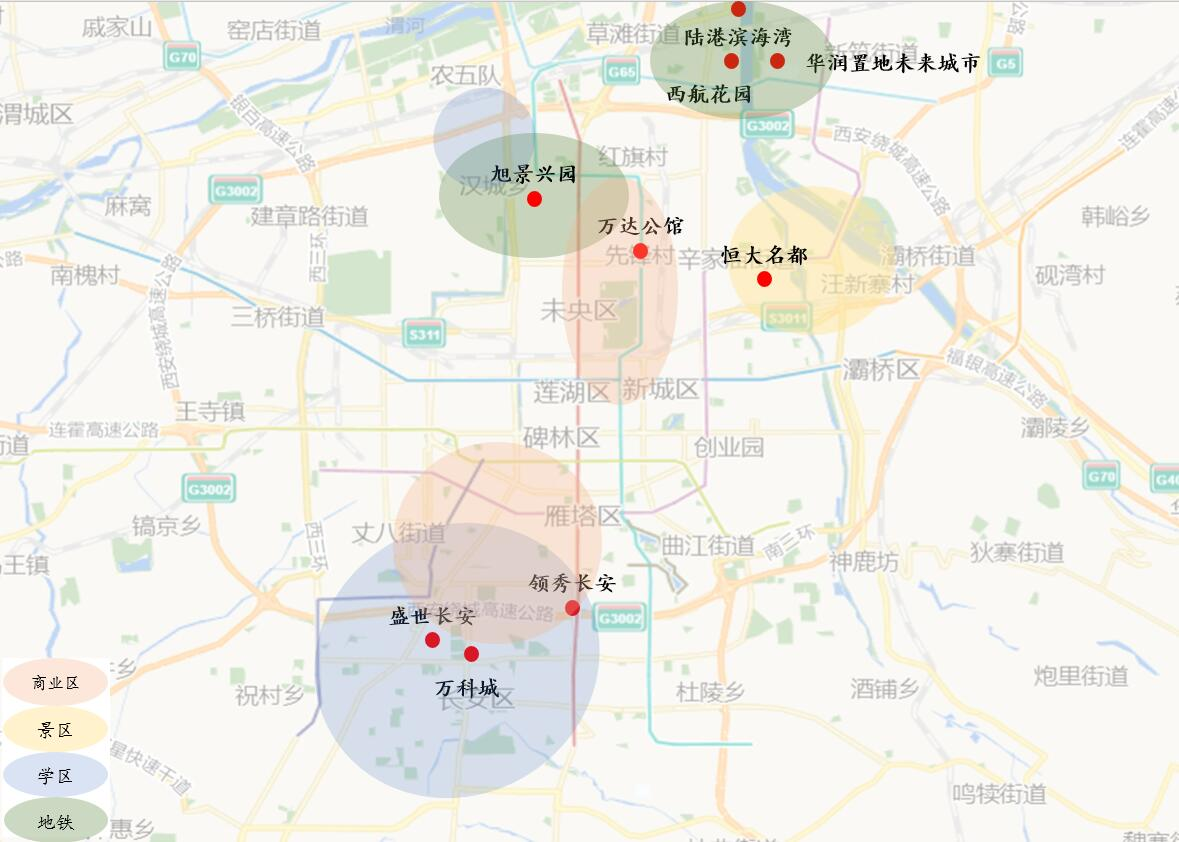
\includegraphics[scale=0.4]{地图.jpg}
    \caption{抽样小区地理因素分布图}
    \label{fig:抽样小区地理因素分布图}
\end{figure}
事实上,在刚刚的模型结果中,5月房价预测值与实际值偏差略大的小区均在这些能对房价产生较大影响的重点地区覆盖下,这说明了将地理因素量化为指标、加入模型评估体系的必要性,下面我们就来实现这一点。

首先,不难发现在被抽样的三个行政区中,长安区公共交通便利且被商圈等要素覆盖程度高,这与位于该区学区、商业区覆盖下的万科城和盛世长安小区平均二手房价较高的特点是相符的。同理,我们可以得出“重点区域覆盖程度较高的小区房屋普遍单价较高”的规律。因而可以通过行政区平均房价的高低反映这一地区被重点区域的覆盖程度,即反映了处于这一地区二手房的地理因素是否优越。具体考量如下:

首先通过附件一所给数据,计算西安12个行政区的平均房价。
\begin{figure}[H]
    \centering
    \begin{tabular}{cccccc}
    \toprule
    编号&区 & 平均房价:元/$m^2$&编号&区&平均房价:元/$m^2$\\
    \midrule
        1&未央区 & 14563 &7&长安区 & 16810 \\
        2&雁塔区 & 14132 &8&高新区 & 19791 \\
        3&莲湖区 & 14129 &9&经开区 & 15020 \\
        4&碑林区 & 16434 &10&国际港务区 & 13918 \\
        5&新城区 & 12996 &11&西咸新区  & 15301 \\
        6&灞桥区 & 13029 &12&浐灞生产区 & 16810 \\
    \bottomrule
    \end{tabular}
    \caption{平均房价}
\end{figure}

再分别计算每个行政区房屋每平米单价的加权平均值。记每一区平均房价为$c_i$,令$x_i=c_i/\sum_{i=1}^{12}c_i$。这样就可以得到归一化的赋值。因而可以将这项指标作为反映房屋地理因素的自变量加入到模型的考量,以实现模型的再改进。

\section{任务三:预测与分析}
\subsection{政策驱动作用}
西安关于调整商品住房交易政策有关问题的通知主要包含:(1)保障合理住房需求;(2)促进二手住房流通;(3)强化住房金融支持;(4)优化个类人群购房政策。

下面我们针对每条通知,具体分析其变化可能对不同外界因素产生的影响,进而分析这些外界因素可能对模型中房屋的11个影响指标造成的间接影响。

(1)保障合理住房要求主要体现在对市外迁入本市户籍的居民家庭和非本市户籍居民家庭的限制购买上,而限购的措施可以抑制房价价格上升,使得房价尽量保持平稳,同时也有降低房价,使房价更加合理的效果\cite{RN3}。另一方面,这样的政策驱动更利于吸引有购房需求与购买力的市外人员落户西安,增加西安常住人才数量,改善西安劳动力结构。

(2)促进二手住房流通,主要措施为:无论是已购买或新购买的是商品住房还是二手住房,均规定房屋产权人在取得《不动产权证书》满两年后方可上市交易。促进二手房流通可以增加市场上二手房交易数量,在一定程度上降低二手房房地产的价格\cite{RN4},同时促进二手房流通也能一定程度上提高二手房的成交量。

(3)强化住房金融支持的具体措施分为以下几类:(i)降低自住房和住房公积金贷款首付比例与年化利率,(ii)将住房公积金贷款额度比例与房屋面积和申请次数挂钩,(iii)规定住房公积金贷款额度上限。这样的举措利好有自住房需求的工作者购买144平方米及以下的普通住房,同时一定程度上限制了利用住房公积金实现多套房屋空置投资的行为,有利于实现房地产业良性循环和健康发展,满足更多市民的住房需求。此外相对而言,这项通知可以一定程度上提升市场对于小面积、小户型、低总价房产的需求量,继而落实到此前模型中的基本指标。

(4)优化各类人群购房政策。优化各类人群购房政策的主要内容为:
(i)在陕院士或其单位用于保障在陕院士居住以及经过市委人才办确认的人才购买商品住房的,予以保障。(ii)西安消防救援人员购买住房、二孩及以上家庭购买商品住房、28周岁及以上未婚者在购买首套商品住房时予以优待。

因此,综合考量这项政策通知,我们认为这次政策将会促进二手房房价的增长,同时促进二手房的流通和成交量的提高,下面进行具体的预测和分析。
\subsection{价格及成交量走势预测}
首先进行二手房价格预测,我们根据收集到的西安市2020年至2022年5月二手房每平方米价格数据\cite{RN5},绘出图表:
\begin{figure}[H]
    \centering
    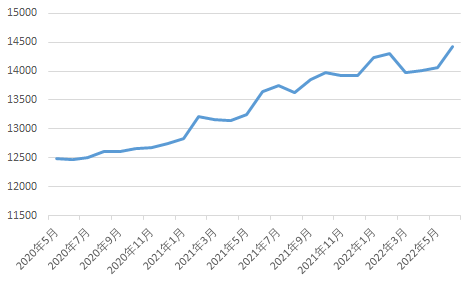
\includegraphics[scale=0.7]{房价变化走势.png}
    \caption{房价变化走势}
    \label{fig:房价变化走势}
\end{figure}

我们建立对数预测模型,原因如下:

首先,根据图像,我们假定,二手房价在总体上是在上涨的。又二手房作为一种商品,它的价格、成交量都受消费者购买力的影响,我们认为,当二手房房价过高时,人们由于购买不足,无法购买二手房导致成交量下降,此时二手房房价的增速放缓。因此,假设每平方米的价格$c$与月份$t$成对数关系,也就是
\begin{equation}
    c(t)=a\ln t+b.
\end{equation}
应用相应的数据得到的拟合结果为:
\begin{table}[H]
  \centering
    \begin{tabular}{cc}
    \toprule
    截距$b$    & 11750.42171 $\pm $ 180.94686 \\
    斜率$a$    & 695.29632 $\pm$ 72.51361 \\
    残差平方和 & 2214778.691 \\
    Pearson's r & 0.8905 \\
    R平方(COD) & 0.793 \\
    调整后R平方 & 0.78437 \\
    \bottomrule
    \end{tabular}%
    \caption{对数预测模型拟合结果}
\end{table}%

结合上面对于西安利好二手房交易政策的出台,我们认为:
首先,由于房屋限购政策的存在,二手房价格的提升不会特别明显,但在西安关于调整商品住房交易政策有关问题的通知中相关的政策颁布之后,我们认为由于政策保障合理的住房需求使得限购措施逐步放宽,再加上通知中合理安置人才的措施对房价的刺激作用,二手房价将会发生增长\cite{RN3},由于政策影响时间比较长,所以,我们认西安二手房房价总体上成上升趋势,又根据第二问以及图(\ref{fig:房价变化走势}),房价上升同时,由于人们购买力限制,二手房价会出现增长速度放缓的现象,而经过进一步计算和对数据的分析处理,我们发现对数预测模型确实拟合情况较好。

接下面对西安下一年的二手房成交量进行预测。

由于人们的可支配资金是有限的,因而随着房价的上升,当房价超过购买力时,西安市的二手房成交量和二手房每平方米价格大约成负相关关系\cite{RN6};而当房价在购买力承受范围内时,房价的提高作用在人们的观念上,致使更多有意购房者预期未来房价升高,继而促进成交量的提高。故综合考量政策通知对住房金融支持的强化作用,我们认为二手房成交量会在一定时期内得到提高。

综上,我们认为西安二手房屋价格在一定时期内总体呈增速放缓的上升趋势,并根据任务二的结果,可能由于交易市场的周期性因素伴有轻微的波动。在房价上升阶段,伴随预期未来房价的升高,无论购房者出于居住刚需还是对投资升值的考量,都可能选择在这一段时间内购房,因此二手房的成交量总体会呈现上升趋势。

\section{模型的评价与推广}
\subsection{优点}

1,评价指标足够充分,样本数量充足。

2,评价方法足够客观。我们先用SPSS将各个评价指标做标准化处理,防止取值数量及差距过于悬殊。之后,我们用主成分分析法来确定各个指标的权重。能够客观的反映各个指标的重要程度进而得到比较客观的评价体系。

\subsection{缺点}

1、在进行层分析法时,对不同指标之间的重要程度对比存在一定主观性。

2、我们忽视了现实生活中不同方向政策难免相互影响的事实,只从数学层面验证了各项指标的线性无关性。

\subsection{模型的推广}

1、在构建多元线性回归方程的评估模型时,利用神经元多输入单输出的特性,我们可以尝试使用神经网络优化模型。

2、在模型的检验时,结合模型的性能度量,考虑模型的精度,通过做pr曲线可以更加直观准确地衡量模型性能。


\bibliographystyle{gbt7714-numerical}
\bibliography{example}

\newpage

\begin{appendices}
    \section{MATLAB程序}

    \subsection{diff\_view\_of\_data.m}

    \begin{lstlisting}[language=MATLAB]
        A=xlsread('data.xlsx');
        W=xlsread('weight_t3.xlsx');
        X=A*W;%纵维度为3
        y=xlsread('price_C.xlsx');
        x1=X(:,1);
        x2=X(:,2);
        x3=X(:,3);
        %% Create figure with 3 subplots
        f = figure('Units','normalized','OuterPosition',[0 .5 1 .5]);
        ax0 = subplot(2,2,1);
        ax1 = subplot(2,2,2);
        ax2 = subplot(2,2,3);
        ax3 = subplot(2,2,4);
        %% Plot some surfaces on 1st subplot
        s=scatter3(ax0,x1,x2,x3,5,y);
        title(ax0,'view(54.7°,54.7°,54,7°)')
        hold(ax0,'on');
        plotObjs =s;
        %% Copy plot objects to other 2 subplots
        copyobj(plotObjs,ax1);
        copyobj(plotObjs,ax2);
        copyobj(plotObjs,ax3);
        %% Set different viewing angle for each subplot
        view(ax1,0,90); title(ax1,'view(90°,90°,0°)');
        view(ax2,90,0); title(ax2,'view(0°,90°,90°)');
        view(ax3,0,0); title(ax3,'view(90°,0°,90°)');
        xlabel(ax0,'x1');ylabel(ax0,'x2');zlabel(ax0,'x3');
        xlabel(ax1,'x1');ylabel(ax1,'x2');zlabel(ax1,'x3');
        xlabel(ax2,'x1');ylabel(ax2,'x2');zlabel(ax2,'x3');
        xlabel(ax3,'x1');ylabel(ax3,'x2');zlabel(ax3,'x3');
        ch = colorbar('horiz');% 横向坐标轴
        set(ch,'position',[0.135 0.035 0.75 0.015],'ticks',(-1:0.2:1),'ticklength',0.015,'fontsize',10,'ticklabels',
        {'<-1.0',(-0.8:0.2:0.8),'>1.0'}) % colorbar的位置,[左 下 宽 高]
    \end{lstlisting}

    \subsection{divide\_group.m}

    \begin{lstlisting}[language=MATLAB]
        A=xlsread('data.xlsx');
        W=xlsread('weight_t3.xlsx');
        X=A*W;%纵维度为3
        y=pdist(X,'mahalanobis');
        ys=squareform(y);
        z=linkage(y);endrogram(z,0);
        T=cluster(z,'cutoff',5,'depth',1000);
    \end{lstlisting}

    \section{SPSS交互命令}

    \begin{lstlisting}[language=MATLAB]
        GET DATA 
        /TYPE=XLSX 
        /FILE='.\支撑材料\链家西安在售二手房数据处理后中间结果.xlsx' 
        /SHEET=name 'sheet1' 
        /CELLRANGE=FULL 
        /READNAMES=ON 
        /DATATYPEMIN PERCENTAGE=95.0 
        /HIDDEN IGNORE=YES. 
      EXECUTE. 
      DATASET NAME 数据集1 WINDOW=FRONT.
      
      FACTOR 
        /VARIABLES Z总价万元 Z所在楼层 Z建筑面积㎡ Z房屋朝向 Z梯户比 Z装修情况 Z供暖方式 Z是否有抵押
        /MISSING LISTWISE 
        /ANALYSIS Z总价万元 Z所在楼层 Z建筑面积㎡ Z房屋朝向 Z梯户比 Z装修情况 Z供暖方式 Z是否有抵押
        /PRINT INITIAL CORRELATION SIG KMO EXTRACTION ROTATION FSCORE 
        /PLOT EIGEN ROTATION 
        /CRITERIA MINEIGEN(1) ITERATE(25) 
        /EXTRACTION PC 
        /CRITERIA ITERATE(25) 
        /ROTATION VARIMAX 
        /SAVE REG(ALL) 
        /METHOD=CORRELATION. 
    \end{lstlisting}

    \section{Jupyter代码}

    \begin{lstlisting}[language=Python]
        {
            "cells": [
             {
              "cell_type": "code",
              "execution_count": 2,
              "id": "b7f10c17",
              "metadata": {},
              "outputs": [
               {
                "data": {
                 "text/html": [
                  "<div>\n",
                  "<style scoped>\n",
                  "    .dataframe tbody tr th:only-of-type {\n",
                  "        vertical-align: middle;\n",
                  "    }\n",
                  "\n",
                  "    .dataframe tbody tr th {\n",
                  "        vertical-align: top;\n",
                  "    }\n",
                  "\n",
                  "    .dataframe thead th {\n",
                  "        text-align: right;\n",
                  "    }\n",
                  "</style>\n",
                  "<table border=\"1\" class=\"dataframe\">\n",
                  "  <thead>\n",
                  "    <tr style=\"text-align: right;\">\n",
                  "      <th></th>\n",
                  "      <th>tab</th>\n",
                  "      <th>esf_jiage</th>\n",
                  "      <th>ptb151</th>\n",
                  "      <th>编号2</th>\n",
                  "      <th>字段</th>\n",
                  "      <th>字段1</th>\n",
                  "    </tr>\n",
                  "  </thead>\n",
                  "  <tbody>\n",
                  "    <tr>\n",
                  "      <th>0</th>\n",
                  "      <td>建筑年代:1996年</td>\n",
                  "      <td>66.96㎡</td>\n",
                  "      <td>发布时间:2022/7/1 16:58:31</td>\n",
                  "      <td>2.201478e+09</td>\n",
                  "      <td>糜家桥小区\\n                                       ...</td>\n",
                  "      <td>2-1-1-1 | 低层/7层 | 东南  建筑年代:1996年</td>\n",
                  "    </tr>\n",
                  "    <tr>\n",
                  "      <th>1</th>\n",
                  "      <td>建筑年代:1998年</td>\n",
                  "      <td>34.42㎡</td>\n",
                  "      <td>发布时间:2022/7/1 16:57:11</td>\n",
                  "      <td>2.201478e+09</td>\n",
                  "      <td>尚德路139号21幢\\n                                  ...</td>\n",
                  "      <td>1-1 | 低层/2层 | 南  建筑年代:1998年</td>\n",
                  "    </tr>\n",
                  "    <tr>\n",
                  "      <th>2</th>\n",
                  "      <td>建筑年代:2006年</td>\n",
                  "      <td>79.34㎡</td>\n",
                  "      <td>发布时间:2022/7/1 16:55:37</td>\n",
                  "      <td>2.201478e+09</td>\n",
                  "      <td>公安五处\\n                                        ...</td>\n",
                  "      <td>3-1-1-1 | 低层/6层 | 南北  建筑年代:2006年</td>\n",
                  "    </tr>\n",
                  "    <tr>\n",
                  "      <th>3</th>\n",
                  "      <td>建筑年代:2012年</td>\n",
                  "      <td>53.85㎡</td>\n",
                  "      <td>发布时间:2022/7/1 16:51:34</td>\n",
                  "      <td>2.201478e+09</td>\n",
                  "      <td>紫郡长安\\n                                        ...</td>\n",
                  "      <td>1-0-1 | 低层/32层 | 北  建筑年代:2012年</td>\n",
                  "    </tr>\n",
                  "    <tr>\n",
                  "      <th>4</th>\n",
                  "      <td>建筑年代:2009年</td>\n",
                  "      <td>127.78㎡</td>\n",
                  "      <td>发布时间:2022/7/1 16:48:53</td>\n",
                  "      <td>2.201478e+09</td>\n",
                  "      <td>欣心家园\\n                                        ...</td>\n",
                  "      <td>3-2-1-2 | 中层/18层 | 南北  建筑年代:2009年</td>\n",
                  "    </tr>\n",
                  "  </tbody>\n",
                  "</table>\n",
                  "</div>"
                 ],
                 "text/plain": [
                  "          tab esf_jiage                  ptb151           编号2  \\\n",
                  "0  建筑年代:1996年    66.96㎡  发布时间:2022/7/1 16:58:31  2.201478e+09   \n",
                  "1  建筑年代:1998年    34.42㎡  发布时间:2022/7/1 16:57:11  2.201478e+09   \n",
                  "2  建筑年代:2006年    79.34㎡  发布时间:2022/7/1 16:55:37  2.201478e+09   \n",
                  "3  建筑年代:2012年    53.85㎡  发布时间:2022/7/1 16:51:34  2.201478e+09   \n",
                  "4  建筑年代:2009年   127.78㎡  发布时间:2022/7/1 16:48:53  2.201478e+09   \n",
                  "\n",
                  "                                                  字段  \\\n",
                  "0  糜家桥小区\\n                                       ...   \n",
                  "1  尚德路139号21幢\\n                                  ...   \n",
                  "2  公安五处\\n                                        ...   \n",
                  "3  紫郡长安\\n                                        ...   \n",
                  "4  欣心家园\\n                                        ...   \n",
                  "\n",
                  "                                 字段1  \n",
                  "0   2-1-1-1 | 低层/7层 | 东南  建筑年代:1996年  \n",
                  "1        1-1 | 低层/2层 | 南  建筑年代:1998年  \n",
                  "2   3-1-1-1 | 低层/6层 | 南北  建筑年代:2006年  \n",
                  "3     1-0-1 | 低层/32层 | 北  建筑年代:2012年  \n",
                  "4  3-2-1-2 | 中层/18层 | 南北  建筑年代:2009年  "
                 ]
                },
                "execution_count": 2,
                "metadata": {},
                "output_type": "execute_result"
               }
              ],
              "source": [
               "import pandas as pd\n",
               "data=pd.read_excel(\"data.xls\")\n",
               "result=pd.DataFrame()\n",
               "data.head(5)\n"
              ]
             },
             {
              "cell_type": "code",
              "execution_count": 4,
              "id": "70395b4f",
              "metadata": {},
              "outputs": [
               {
                "name": "stderr",
                "output_type": "stream",
                "text": [
                 "C:\\Users\\sp\\AppData\\Local\\Temp\\ipykernel_42916\\59496173.py:12: FutureWarning: As the xlwt package is no longer maintained, the xlwt engine will be removed in a future version of pandas. This is the only engine in pandas that supports writing in the xls format. Install openpyxl and write to an xlsx file instead. You can set the option io.excel.xls.writer to 'xlwt' to silence this warning. While this option is deprecated and will also raise a warning, it can be globally set and the warning suppressed.\n",
                 "  result.to_excel(\"数据.xls\")\n"
                ]
               }
              ],
              "source": [
               "result['年代']=data.iloc[:,0].str.split(\":\",expand=True)[1].str.
               split(\"年\",expand=True)[0]\n",
               "result['面积']=data.iloc[:,1].str.split(\"㎡\",expand=True)[0]\n",
               "result['发布时间']=data.iloc[:,2].str.split(\":\",expand=True)[1]\n",
               "result['编号']=data.iloc[:,3].astype(\"str\").str.split(\".\",expand=True)[0]\n",
               "result['地址']=data.iloc[:,4].str.split(\"\\n\",expand=True)[0]\n",
               "result['详细住址']=data.iloc[:,4].str.split(\"\\n\",expand=True)[1].str.strip()
               \n",
               "result['户型']=data.iloc[:,5].str.split(\" | \",expand=True)[0]\n",
               "result['楼层类型']=data.iloc[:,5].str.split(\" | \",expand=True)[2].str.split(\"/\",expand=True)[0]\n",
               "result['楼层']=data.iloc[:,5].str.split(\" | \",expand=True)[2].str.split(\"/\",expand=True)[1].
               str.split(\"层\",expand=True)[0]\n",
               "result['朝向']=data.iloc[:,5].str.split(\" | \",expand=True)[4].str.split(\"  \",expand=True)[0]\n",
               "result['建筑日期']=data.iloc[:,5].str.split(\":\",expand=True)[1].str.split
               (\"年\",expand=True)[0]\n",
               "result.to_excel(\"数据.xls\")"
              ]
             },
             {
              "cell_type": "code",
              "execution_count": 23,
              "id": "b83e442a",
              "metadata": {},
              "outputs": [
               {
                "data": {
                 "text/html": [
                  "<div>\n",
                  "<style scoped>\n",
                  "    .dataframe tbody tr th:only-of-type {\n",
                  "        vertical-align: middle;\n",
                  "    }\n",
                  "\n",
                  "    .dataframe tbody tr th {\n",
                  "        vertical-align: top;\n",
                  "    }\n",
                  "\n",
                  "    .dataframe thead th {\n",
                  "        text-align: right;\n",
                  "    }\n",
                  "</style>\n",
                  "<table border=\"1\" class=\"dataframe\">\n",
                  "  <thead>\n",
                  "    <tr style=\"text-align: right;\">\n",
                  "      <th></th>\n",
                  "      <th>标题</th>\n",
                  "      <th>positionInfo</th>\n",
                  "      <th>houseInfo</th>\n",
                  "      <th>followInfo</th>\n",
                  "      <th>totalPrice</th>\n",
                  "      <th>unitPrice</th>\n",
                  "      <th>详情标题</th>\n",
                  "      <th>日期时间</th>\n",
                  "      <th>字段1</th>\n",
                  "      <th>字段2</th>\n",
                  "      <th>...</th>\n",
                  "      <th>字段12</th>\n",
                  "      <th>字段13</th>\n",
                  "      <th>字段14</th>\n",
                  "      <th>字段15</th>\n",
                  "      <th>字段16</th>\n",
                  "      <th>字段17</th>\n",
                  "      <th>字段18</th>\n",
                  "      <th>字段19</th>\n",
                  "      <th>字段20</th>\n",
                  "      <th>字段21</th>\n",
                  "    </tr>\n",
                  "  </thead>\n",
                  "  <tbody>\n",
                  "    <tr>\n",
                  "      <th>0</th>\n",
                  "      <td>车城温泉花园 2室2厅 南 北</td>\n",
                  "      <td>车城温泉花园    -  高陵</td>\n",
                  "      <td>2室2厅 | 112.89平米 | 南 北 | 简装 | 6层  | 板塔结合</td>\n",
                  "      <td>2人关注 / 6天以前发布</td>\n",
                  "      <td>76.0</td>\n",
                  "      <td>6,733元/平</td>\n",
                  "      <td>车城温泉花园 2室2厅 南 北</td>\n",
                  "      <td>2022-06-25</td>\n",
                  "      <td>76.0</td>\n",
                  "      <td>6733元/平米</td>\n",
                  "      <td>...</td>\n",
                  "      <td>装修情况简装</td>\n",
                  "      <td>供暖方式集中供暖</td>\n",
                  "      <td>配备电梯无</td>\n",
                  "      <td>挂牌时间\\n                              2022-06-25</td>\n",
                  "      <td>交易权属\\n                              商品房</td>\n",
                  "      <td>上次交易\\n                              2007-11-07</td>\n",
                  "      <td>房屋用途\\n                              普通住宅</td>\n",
                  "      <td>房屋年限\\n                              满五年</td>\n",
                  "      <td>产权所属\\n                              共有</td>\n",
                  "      <td>抵押信息\\n                              \\n        ...</td>\n",
                  "    </tr>\n",
                  "  </tbody>\n",
                  "</table>\n",
                  "<p>1 rows × 29 columns</p>\n",
                  "</div>"
                 ],
                 "text/plain": [
                  "                标题     positionInfo                                houseInfo  \\\n",
                  "0  车城温泉花园 2室2厅 南 北  车城温泉花园    -  高陵  2室2厅 | 112.89平米 | 南 北 | 简装 | 6层  | 板塔结合   \n",
                  "\n",
                  "      followInfo  totalPrice unitPrice             详情标题        日期时间   字段1  \\\n",
                  "0  2人关注 / 6天以前发布        76.0  6,733元/平  车城温泉花园 2室2厅 南 北  2022-06-25  76.0   \n",
                  "\n",
                  "        字段2  ...    字段12      字段13   字段14  \\\n",
                  "0  6733元/平米  ...  装修情况简装  供暖方式集中供暖  配备电梯无   \n",
                  "\n",
                  "                                             字段15  \\\n",
                  "0  挂牌时间\\n                              2022-06-25   \n",
                  "\n",
                  "                                      字段16  \\\n",
                  "0  交易权属\\n                              商品房   \n",
                  "\n",
                  "                                             字段17  \\\n",
                  "0  上次交易\\n                              2007-11-07   \n",
                  "\n",
                  "                                       字段18  \\\n",
                  "0  房屋用途\\n                              普通住宅   \n",
                  "\n",
                  "                                      字段19  \\\n",
                  "0  房屋年限\\n                              满五年   \n",
                  "\n",
                  "                                     字段20  \\\n",
                  "0  产权所属\\n                              共有   \n",
                  "\n",
                  "                                                字段21  \n",
                  "0  抵押信息\\n                              \\n        ...  \n",
                  "\n",
                  "[1 rows x 29 columns]"
                 ]
                },
                "execution_count": 23,
                "metadata": {},
                "output_type": "execute_result"
               }
              ],
              "source": [
               "import pandas as pd\n",
               "data2=pd.read_excel(\"原始数据_西安二手房房源.xlsx\")\n",
               "data2.head(1)"
              ]
             },
             {
              "cell_type": "code",
              "execution_count": 35,
              "id": "20d87384",
              "metadata": {},
              "outputs": [
               {
                "name": "stderr",
                "output_type": "stream",
                "text": [
                 "C:\\Users\\sp\\AppData\\Local\\Temp\\ipykernel_36436\\3555151398.py:27: FutureWarning: As the xlwt package is no longer maintained, the xlwt engine will be removed in a future version of pandas. This is the only engine in pandas that supports writing in the xls format. Install openpyxl and write to an xlsx file instead. You can set the option io.excel.xls.writer to 'xlwt' to silence this warning. While this option is deprecated and will also raise a warning, it can be globally set and the warning suppressed.\n",
                 "  result2.to_excel(\"二手房信息.xls\")\n"
                ]
               }
              ],
              "source": [
               "result2=pd.DataFrame()\n",
               "result2['小区名']=data2.iloc[:,0].str.split(\" \",expand=True)[0]\n",
               "result2['所在区域']=data2.iloc[:,1].str.split(\"-\",expand=True)[1].
               str.strip()\n",
               "result2['户型']=data2.iloc[:,2].str.split(\"|\",expand=True)[0]\n",
               "result2['面积']=data2.iloc[:,2].str.split(\"|\",expand=True)[1].str.split
               (\"平米\",expand=True)[0]\n",
               "result2['朝向']=data2.iloc[:,2].str.split(\"|\",expand=True)[2]\n",
               "result2['装修']=data2.iloc[:,2].str.split(\"|\",expand=True)[3]\n",
               "result2['楼层']=data2.iloc[:,13].str.split(\"/\",expand=True)[0]\n",
               "result2['总共楼层']=data2.iloc[:,13].str.split(\"/\",expand=True)[1]\n",
               "result2['建筑类型']=data2.iloc[:,2].str.split(\"|\",expand=True)[5]\n",
               "result2['关注人数']=data2.iloc[:,3].str.split(\"人\",expand=True)[0]\n",
               "result2['房价(万)']=data2.iloc[:,4]\n",
               "result2['每平米房价']=data2.iloc[:,5].str.split(\"元\",expand=True)[0]\n",
               "result2['挂牌时间']=data2.iloc[:,7]\n",
               "result2['户型结构']=data2.iloc[:,18].str.split(\"户型结构\",expand=True)[1].
               str.strip()\n",
               "result2['装修情况']=data2.iloc[:,19].str.split(\"装修情况\",expand=True)[1].
               str.strip()\n",
               "result2['供暖方式']=data2.iloc[:,20].str.split(\"供暖方式\",expand=True)[1].
               str.strip()\n",
               "result2['配备电梯']=data2.iloc[:,21].str.split(\"配备电梯\",expand=True)[1].
               str.strip()\n",
               "result2['交易权属']=data2.iloc[:,23].str.split(\"交易权属\",expand=True)[1].
               str.strip()\n",
               "result2['配备电梯']=data2.iloc[:,21].str.split(\"配备电梯\",expand=True)[1].
               str.strip()\n",
               "result2['上次交易']=data2.iloc[:,24].str.split(\"上次交易\",expand=True)[1].
               str.strip()\n",
               "result2['房屋用途']=data2.iloc[:,25].str.split(\"房屋用途\",expand=True)[1].
               str.strip()\n",
               "result2['房屋年限']=data2.iloc[:,26].str.split(\"房屋年限\",expand=True)[1].
               str.strip()\n",
               "result2['产权所属']=data2.iloc[:,27].str.split(\"产权所属\",expand=True)[1].
               str.strip()\n",
               "result2['抵押信息']=data2.iloc[:,28].str.split(\"抵押信息\",expand=True)[1].
               str.strip()\n",
               "result2.to_csv(\"二手房信息.csv\")\n",
               "result2.to_excel(\"二手房信息.xls\")"
              ]
             },
             {
              "cell_type": "code",
              "execution_count": null,
              "id": "2820a1fe",
              "metadata": {},
              "outputs": [],
              "source": []
             }
            ],
            "metadata": {
             "kernelspec": {
              "display_name": "Python 3.10.4 64-bit",
              "language": "python",
              "name": "python3"
             },
             "language_info": {
              "codemirror_mode": {
               "name": "ipython",
               "version": 3
              },
              "file_extension": ".py",
              "mimetype": "text/x-python",
              "name": "python",
              "nbconvert_exporter": "python",
              "pygments_lexer": "ipython3",
              "version": "3.10.4"
             },
             "vscode": {
              "interpreter": {
               "hash": "28b3b17067e4930633005eb39e548462d5e9437e6c9b4c2b70295c23a85f602c"
              }
             }
            },
            "nbformat": 4,
            "nbformat_minor": 5
           }           
    \end{lstlisting}
\end{appendices}

\end{document}
